\documentclass{article}
\input ../preamble
\parindent = 0em

%\newcommand{\solution}[1]{}
\newcommand{\solution}[1]{\bigskip {\color{red} {\bf Solution}: #1}}

\begin{document}


\centerline{\bf TTIC 31230 Fundamentals of Deep Learning, 2020}
\medskip
\centerline{\bf Problems For Language Modeling, Translation and Attention.}

\bigskip

{\bf Problem 1. Blank Language modeling.} This problem considers ``blank language modeling'' which is used in BERT.
For blank language modelng we draw a sentence $w_1,\ldots,w_T$ from a corpose and blank out a word at random
and ask the system to predict the blanked word.  The cross-entropy loss for blank language modeling can be written as
$$\Phi^* = \argmin_\Phi\;E_{w_1,\ldots,w_T \sim \mathrm{Train}, t \sim \{1,\ldots,T\}}\;\;- \ln P_\Phi(w_t| w_1,\ldots,w_{t-1},w_{t+1},\ldots,w_T)$$
    
Consider a bidirectional RNN run on a sequence of words $w_1,\ldots,w_T$ such that for each time $t$ we have a forward
hidden state $\vec{h}[t,J]$ computed from $w_1,\ldots,w_t$ and a backward hidden state $\cev{h}[t,J]$ computed from $w_T,\;w_{T-1},\ldots w_t$.
Also assume that each word $w$ has an associated word vector $e[w,J]$.
Give a definition of $P(w_t\;|\;w_1,\ldots w_{t-1},\;w_{t+1},\ldots,w_T)$ as a function of
the vectors $\vec{h}[t-1,J]$ and $\cev{h}[t+1,J]$ and the word vectors $e[W,I]$.
You can assume that $\vec{h}[T,J]$ and $\cev[h][T,J]$ have the same shape (same dimensions) but
do not make any assumptions about the dimension of the word vectors $e[W,I]$.
You can assume whatever tensor parameters you want.

\solution{
  There are various acceptable solutions.  A simple one is to assume the parameters include matrices  $\vec{W}[I,J]$ and $\cev{W}[I,J]$.
  Using this convention and the standard convention for matrix-vector products we can then write a solution as
  \begin{eqnarray*}
    & & P_\Phi(w_t| w_1,\ldots,w_{t-1},w_{t+1},\ldots,w_T) \\
    & = & \softmax_{w_t} \;\;e[w_t,I]\vec{W}[I,J]\vec{h}[t-1,J]\; + \; e[w_t,I]\cev{W}[I,J]\cev{h}[t+1,J]
  \end{eqnarray*}
}

\bigskip
{\bf Problem 2. Image Captioning as Translation with Attention.} In machine translation with attention the translation is generated from an autoregressive language model for the target langauge translation given the source language sentence.
The source sentence is converted to an initial hidden vector $h[0,J]$ for the decoding (usually the final hidden vector of a right-to-left RNN run on the input), plus the sequence
$M[T_{\mathrm{in}},J]$ of hidden vectors computed by the RNN on the source sentence where $T$ is the length of the source sentence.  We then define an autoregressive conditional language model
$$P_\Phi(w_1,\ldots,w_{T_\mathrm{out}}\;|\; h[0,J],\;M[T_{\mathrm{in}},J])$$
An autoregressive conditional language model with attention can be defined by
\begin{eqnarray*}
P(w_t\;|\;w_0,\cdots,w_{t-1}) & = & \softmax_{w_t}\;e[w_t,I]W^{\mathrm{auto}}[I,J]h[t-1,J] \\
\\
\alpha[t_{\mathrm{in}}]& =& \softmax_{t_\mathrm{in}} \;h[t\!-\!1,J_1]W^{\mathrm{key}}[J_1,J_2]M[t_{\mathrm{in}},J_2]\\
\\
V[J]& = & \sum_{t_{\mathrm{in}}}\;\alpha[t_{\mathrm{in}}]M[t_{\mathrm{in}},J] \\
\\
h[t,J] & = & \mathrm{CELL}_\Phi (h[t-1,J],\;V[J],\;e[w_t,I])
\end{eqnarray*}
Here $\mathrm{CELL}$ is some function taking (objects for) two vectors of dimensions J and one vector of dimension I and returning (an object for) a vector of dimension $J$.

\medskip
Rewrite these equations for image captioning where instead of $M[t_{\mathrm{in}},J]$ we are given an image feature tensor $M[x,y,K]$

\solution{
\begin{eqnarray*}
P(w_t\;|\;w_0,\cdots,w_{t-1}) & = & \softmax_{w_t}\;e[w_t,I]W^{\mathrm{auto}}[I,J]h[t-1,J] \\
\\
\alpha[x,y]& =& \softmax_{x,y} \;h[t\!-\!1,J]W^{\mathrm{key}}[J,K]M[x,y,K]\\
\\
V[K]& = & \sum_{x,y}\;\alpha[x,y]M[x,y,K] \\
\\
h[t,J] & = & \mathrm{CELL}_\Phi (h[t-1,J],\;V[K],\;e[w_t,I])
\end{eqnarray*}
}

\bigskip
{\bf Problem 3. Language CNNs.}
This problem is on CNNs for sentences.  We consider a model with parameters
$$\Phi = (e[w,i], W_1[\Delta t,i,i'], B_1[i],\ldots,W_L[\Delta t,i,i'],B_L[i])$$
The matrix $e$ is the word embedding matrix where $e[w,I]$ is the vector embedding of word $w$.

\medskip
(a) Give an equation for the convolution layer $L_0[b,t,i]$ as a function of the word embeddings and the input sentence $w_1,\ldots,w_T$.

\solution{
  $$L_0[b,t,i] = e[w[b,t],i]$$}

\medskip
(b) Give an equation for $L_{\ell+1}[b,t,i]$ as a function of $L_\ell[b,t,i]$ and the parameters $W_{\ell+1}[\Delta t,i',i]$ and $B_{\ell+1}[i]$
and where $L_{\ell+1}$ is computed stride 2.

\solution{
$$L_{\ell+1}[b,t,i] = \sigma\left(\left(\sum_{\Delta t,i'}\;W_{\ell+1}[\Delta t,i',i]L_\ell[2t + \Delta t,i']\right) - B_{\ell+1}[i]\right)$$
}
  
\medskip
(c) Assuming all computations can be done in parallel as soon the inputs have been computed, what is the {\bf parallel} order
of run time for this convolutional model as a function of the input length $T$ and the number of layers $L$ (assume all parameter tensors
of size $O(1)$). Compare this with the parallel run time of an RNN.

\solution{The CNN has $O(L)$ parallel run time while the RNN is $O(T)$ or $O(T+L)$ with $L$ layers of RNN.}

\bigskip {\bf Problem 4.} A dependency parse is a labeled directed graph on the words in a sentence.
For example,

\centerline{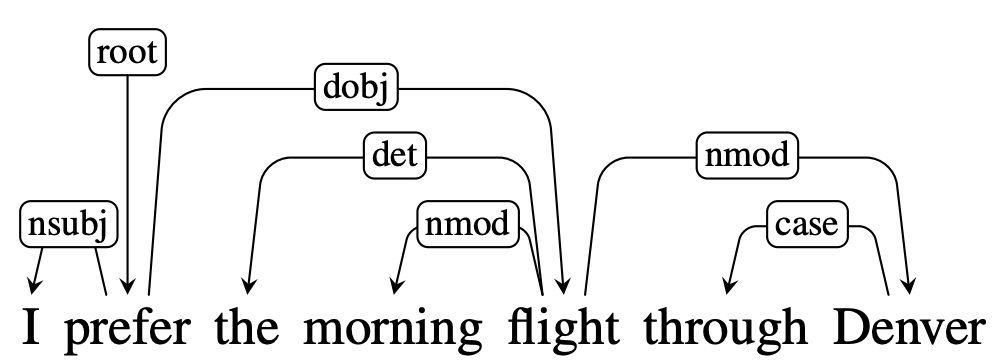
\includegraphics[width = 3in]{/users/davidmcallester/ttic-31230/images/DepParsing.png}}

\medskip
In this example the edges are labeled with {\bf nsubj}, {\bf dobj}, {\bf det}, {\bf nmod} and {\bf case}.
A dependency parse determines a tree with a root node labeled as {\bf root} and with the other nodes labeled with the words of the sentence.
This tree structure defines a set of phrases where each phrase
consists of words beneath a given node of the tree.

\medskip{\bf (a)} Let $k$ range over the set of possible labels in a dependency parse.  There is typically a small fixed set of such labels.
If we interpret $k$ has a transformer head, what attention $\alpha({\mbox{\bf dobj}},{\bf prefer},w)$ over the words $w$ attended from the word {\bf prefer} by the head
{\bf dobj} corresponds to the above dependency parse?

\solution{
  $$\alpha({\bf dobj},{\bf prefer},w) = \left\{\begin{array}{rl} 1 & \mbox{if $w$ is {\bf flight}} \\ 0 & \mbox{otherwise}\end{array}\right.$$
  }

\medskip
{\bf (b)} A dependency parse rarely has two edges leading from a given word that both have the same label.  GTP-3 has 96 heads in each of 96 self-attention layers.
It might be reasonable that, with so many heads, each head chould be encouraged to focus its attention on a small number of words (as would be typical in a dependency parse).
Define a loss ${\cal L}_{\mathrm{focus}}$ that can be combined with the log loss term of the language model such that
${\cal L}_{\mathrm{focus}}$ encourages each head to focus on a small number of words.  Write the total loss as a weighted sum of the language model loss ${\cal L}_{\mathrm{LM}}$
and ${\cal L}_{\mathrm{focus}}$.  You do not need to define ${\cal L}_{\mathrm{LM}}$, just ${\cal L}_\mathrm{focus}$.

\solution{
  \begin{eqnarray*}
    {\cal L}_{\mathrm{total}} & = & {\cal L}_{\mathrm{LM}} + \lambda {\cal L}_{\mathrm{focus}} \\
    \\
      {\cal L}_{\mathrm{focus}} & = & \frac{1}{KTL} \;\sum_{\ell,k,t_1} \;H(k,t_1,T_2) \\
      \\
      & = & \frac{1}{KTL} \sum_{\ell, k,t_1}\;\sum_{t_2} \; \alpha[\ell,k,t_1,t_2] (-\ln \alpha[\ell,k,t_1,t_2])
  \end{eqnarray*}

  The factor of $\frac{1}{KTL}$ can be incorporated into $\lambda$ which is also a correct solution although it introduces a stronger
  coupling of the hyper-parameter $\lambda$ with the size of the transformer model.
}

\medskip
    {\bf (c)} Dependency edges tend to be between nearby words.
    Repeat part {\bf (b)} but for a loss ${\cal L}_{\mathrm{near}}$ which encourages the attention $\alpha[\ell,k,t_1,T_2]$ to be focused near $t_1$.
The loss ${\cal L}_{\mathrm{near}}$ should be ``robust'' in the sense that it has a maximum value that is independent of the length $T$ of the transformer
window.  This should allow some ``outlier'' long distance attentions which are needed for coreference.

\solution{
  \begin{eqnarray*}
    {\cal L}_{\mathrm{total}} & = & {\cal L}_{\mathrm{LM}} + \lambda {\cal L}_{\mathrm{near}} \\
    \\
    {\cal L}_{\mathrm{near}} & = & \frac{1}{KT(L-1)} \sum_{k,t_1,0 \leq \ell \leq L-2}\;\min\left(L_{\mathrm{max}}, \sum_{t_2} \; \alpha[\ell,k,t_1,t_2] (t_1-t_2)^2\right)
  \end{eqnarray*}

  Other solutions are also possible.
}

\medskip
{\bf (d)} State the ``universalty assumption'' under which the ``loss shaping'' terms of {\bf (b)} and ${\bf (c)}$ above only hurts the langauge modeling performance.  Also give a plausibility argument
that these terms might help in practice.

\solution{The universality assumption is that the model parameters will be be optimized so as to find the actual minimum of the loss on the population distribution.  In that case
  the loss shaping terms can only hurt performance.  If, on the other hand, the training does not find the optimal parameters on the population then it seems plausible that the loss shaping terms might help with the optimization or the generalization.}
  

\bigskip
{\bf Problem 5.} For a typical language model the softmax operation defining the probablility $P(w_{t+1}\;|\;w_1,\ldots,w_t)$ has the form
$$\alpha[\ell,t,w] = \softmax_{w} h[\ell,t,I] e[w,I]$$
We now consider adding a ``temperature parameter'' $\beta$ to this softmax.
\begin{equation}
  \alpha[\ell,t,w] = \softmax_{w}\;\; \beta\;h[\ell,t,I] e[w,I] \label{eqlang}
\end{equation}


\medskip
{\bf (a)} Assume that the components of the vector $h[t,I]$ are independent with zero mean and unit variance.  Also assume that that the word vectors have
been initialized so that the components of the vector $e[w,I]$ are zero mean and unit variance.  What initial value of $\beta$ gives the result that
the inner product $\beta h[t,I]e[w,I]$ has zero mean and unit variance. Explain your answer.  (Use $I$ to denote the dimension of the vectors $h[t,I]$ and $w[w,I]$.)

\solution{The mean of a sum of zero mean variables has zero mean.  The standard deviation of a sum of $I$ independent variables each with unit variance
  is $\sqrt{I}$.  Therrefore we get unit variance by setting $\beta = \frac{1}{\sqrt{I}}$.
  }

\medskip
{\bf (b)} Relate your answer to (a) to the equation used for the self attention $\alpha(k,t_1,t_2)$ computed in the tansformer.

\solution{The transformer attention is given by
  $$\alpha[\ell,k,t_1,t_2] = \softmax_{t_2}\; \frac{1}{\sqrt{I}}\;\mathrm{Query}[\ell,k,t_1,I]\mathrm{Key}[\ell,k,t_2,I]$$
  This has the same ``temperature parameter'' as the answer to part (a).}

\bigskip
{\bf Problem 6.} This problem is on transformer self-attention.  Modern classification problems tend to use a softmax operation of the form
\begin{equation}
  P(y|h) = \softmax_y\;h^\top e(y) \label{eqproduct}
\end{equation}
where $h$ is a vector computed by the neural network and $e(y)$ is a vector embedding for the label $y$.  Perhaps five years ago many systems would insert a parameter matrix
so that we have
\begin{equation}
  P(y|h) = \softmax_y\;h^\top W e(y) \label{eqgenprod}
\end{equation}

However, it was generally observed that additional parameterization of the inner product operation does not improve the results.  The vector $h$ and the embedding $e(y)$
can be learned to be such that the standard inner product works well.

However, the attention softmax of the transformer (\ref{eqgenprod}) does not use a naive inner product.

\medskip
    {\bf (a)} Explain why we cannot replace (\ref{eqgenprod}) with a naive inner product of $L[\ell,t_1,J]$ and $L[\ell,t_2,J]$ as in (\ref{eqproduct}).

    \solution{The attention $\alpha[\ell,k,t_1,t_2]$ need to depend on the particular head $k$.  Different heads compute different information as indicated in problem 2.}
    
\medskip
{\bf (b)} Rewrite the transformer self-attention equation (\ref{eqgenprod}) in the form of (\ref{eqgenprod}) where
the matrix $W$ in (\ref{eqgenprod}) is replaced by by a matrix defined in terms of $W^K$ and $W^Q$.

\solution{
  \begin{eqnarray*}
    \alpha[\ell,k,t_1,t_2] & = & \softmax_{t_2}\; \frac{1}{\sqrt{I}}\;L[\ell,t_1,J]\;W^{QK}[\ell,k,J,J']\;L[\ell,t2,J'] \\
    \\
    w^{QK}[\ell,k,j_1,j_2] & = & W^Q[\ell,k,I,j_1]W^K[\ell,k,I,j_2]
  \end{eqnarray*}
}

\medskip
{\bf (c)} Give the number of multiplications computed by the self attention computations (\ref{eqlang}) through (\ref{eqgenprod}) for a single layer $\ell$  and head $k$ as a function of the sequence
length $T$ and vector dimensions $I$ and $J$.  Compare this with the number of multiplications for your solution to (b) assuming that the matrix you introduced is taken to be a parameter matrix of the self attantion as in
(\ref{eqgenprod}).



\solution{
  For equations (\ref{eqlang}) through (\ref{eqgenprod}) we get $2TIJ + T^2I^2$.  For the solution to (a) we get $T^2J^2$.  Since we typically have $I << J$ the solution to (a) is much less efficient.
}


\bigskip {\bf Problem 7.}  Here we consider a neural trigram model.  In a trigram model each word is predicted from the two preceding words using a conditional probability $P_\Phi(w_{t+2}|w_t,w_{t+1})$.
We will assume trained word embeddings $e(w)$ for each word $w$ and a neural network predictor of the form
$$P(w_{t+1}|w_t,w_{t+1}) = \softmax_{w_{t+2}} \beta \; h_\Phi(e(w_t),e(w_{t+1}))^\top\;e(w_{t+2})$$
where $h_\Phi$ is some arbitray neural network returnnig a quey vector and $\beta$ is a temperature parameter.
We will assume that the model has been trained with $\beta$ held fixed at 1 but that we will generate from this trigram model with different values of $\beta$.
What degenerate behavior are we guaranteed to see if we sample at zero temperature?  Explain your answer.

\solution{We are guaranteed to eventually repeat a bigram (a pair of words).  At zero temperature the generation is deterministic
  and hence when a pair of words is repeated we must then see exactly the sequence following the first occurance of that bigram and the generation enters a deterministic loop.
  This happens in practice with many transformer models when sampling at low temperatures.}

\bigskip
{\bf Problem 8.} A self-attention layer in the transformer takes a sequence of vectors $h_\mathrm{in}[T,J]$ and computes
a sequence of vectors $h_\mathrm{out}[T,J]$ using the following equations where $k$ ranges over ``heads''. Heads are intended to allow for
different relationship between words such as ``coreference'' or ``subject of'' for a verb. But the actual meaning emerges during training
and is typically difficult or impossible to interpret.  In the following equations we typically hve $U < J$ and we require $I = J/K$
so that the concatenation of $K$ vectors of dimension $I$ is a vector of dimension $J$.

\begin{eqnarray*}
\mathrm{Query}[k,t,U] & = & W^Q[k,U,J]h_\mathrm{in}[t,J] \\
\\
\mathrm{Key}[k,t,U] & = &  W^K[k,U,J]h_\mathrm{in}[t,J] \\
\\
\alpha[k,t_1,t_2] & = & \softmax_{t_2}\; \mathrm{Query}[k,t_1,U]\mathrm{Key}[k,t_2,U]\\
\\
\mathrm{Value}[k,t,I] & = & W^V[k,I,J]h_\mathrm{in}[t,J] \\
\\
\mathrm{Out}[k,t,I] & = & \sum_{t'}\alpha[k,t,t']\mathrm{Value}[k,t',I] \\
\\
h_\mathrm{out}[t,J] & = & \mathrm{Out}[1,t,I];\cdots;\mathrm{Out}[K,t,I]
\end{eqnarray*}

A summation over $N$ terms can be done in parallel in $O(\log N)$ time.

\medskip
(a) For a given head $k$ and position $t_1$ what is the parallel running time of the above softmax operation, as a function of $T$ and $U$
where we first compute the scores to be used in the softmax and then compute the normalizing constant $Z$.

\solution{
  The scores can be computed in parallel in $\ln U$ time and then $Z$ can be computed in $\ln T$ time.  We then get $O(\ln T + \ln U)$.
  In practice the inner product used in computing the scores would be done in $O(U)$ time giving $O(U + \ln T)$.
}

\medskip
(b) What is the order of running time of the self-attention layer as a function of $T$, $J$ and $K$ (we have $I$ and $U$ are both less than $J$.)

\solution{$O(\ln T + \ln J)$.  In practice the inner products would be done serially which would give $O(J + \ln T)$.}


\bigskip

{\bf Problem 9.}
Just as CNNs can be done in two dimensions for vision and in one dimension for language, the Transformer can be done in two dimensions for vision --- the so-called spatial transformer.

\medskip
(a) Rewrite the equations from problem 1 so that the time index $t$ is replaced by spatial dimensions $x$ and $y$.

\solution{

\begin{eqnarray*}
\mathrm{Query}[k,x,y,U] & = & W^Q[k,U,J]h_\mathrm{in}[x,y,J] \\
\\
\mathrm{Key}[k,x,y,U] & = &  W^K[k,U,J]h_\mathrm{in}[x,y,J] \\
\\
\alpha[k,x_1,y_1,x_2,y_2] & = & \softmax_{x_2,y_2}\; \mathrm{Query}[k,x_1,y_1,U]\mathrm{Key}[k,x_2,y_2,U]\\
\\
\mathrm{Value}[k,x,y,I] & = & W^V[k,I,J]h_\mathrm{in}[x,y,J] \\
\\
\mathrm{Out}[k,x,y,I] & = & \sum_{x',y'}\alpha[k,x,y,x',y']\mathrm{Value}[k,x',y',I] \\
\\
h_\mathrm{out}[x,y,J] & = & \mathrm{Out}[1,x,y,I];\cdots;\mathrm{Out}[K,x,y,I]
\end{eqnarray*}
}

\medskip
(b) Assuming that summations take logarithmic parallel time, give the parallel order of run time for the spatial self-attention layer as a function
of $X$, $Y$, $J$ and $K$ (we have that $I$ and $U$ are both less than $J$).

\solution{$O(\ln XY + \ln J)$}


\bigskip
{\bf Problem 10.} The self-attention in the transformer is computed by the following equations.

\begin{eqnarray*}
\mathrm{Query}_{\ell+1}[k,t,i] & = & W^Q_{\ell+1}[k,i,J]L_\ell[t,J] \\
\\
\mathrm{Key}_{\ell+1}[k,t,i] & = &  W^K_{\ell+1}[k,i,J]L_\ell[t,J] \\
\\
\alpha_{\ell+1}[k,t_1,t_2] & = & \softmax_{t_2}\; \left[\frac{1}{\sqrt{I}}\;\mathrm{Query}_{\ell+1}[k,t_1,I]\mathrm{Key}_{\ell+1}[k,t_2,I]\right]
\end{eqnarray*}

Notice that here the shape of $W^Q$ and $W^K$ are both $[K,I,J]$.  We typically have $I < J$ which makes the inner product in the last line an inner product of lower dimensional vectors.

\medskip
{\bf(a) 20 pts} Give an equation computing a tensor $\tilde{W}^Q[K,J,J]$ computed from $W^Q$ and $W^K$ such that the attention $\alpha(k,t_1,t_2)$ can be written as
$$\alpha_{\ell+1}(k,t_1,t_2) = \softmax_{t_2}\;\left[L_\ell[t_1,J_1]\tilde{W}^Q[k,J_1,J_2]L_\ell[t_2,J_2]\right]$$
For a fixed $k$ we have that $W^Q[k,I,J]$ and $W^K[k,I,J]$ are matrices.  We want a matrix $\tilde{W}^Q[k,J,J]$ such that the attention can be written in matrix notation as
$h_1^\top \tilde{W}^Q h_2$ where $h_1$ and $h_2$ are vectors and $\tilde{W}^Q$ is a matrix.
You need write this matrix $\tilde{W}^Q$ in terms of the matrices for $W^Q$ and $W^K$.  But write your final answer in Einstein notation with $k$ as the first index.

\ignore{
  This is easier to do in vector-matrix notation for a fixed k.  But it can also be done entirely in Einstein notation:
  \begin{eqnarray*}
    & = & \softmax_{t_2} \left[\frac{1}{\sqrt{I}}\;(L_\ell(t_1,J_1)W^Q[k,I,J_1])\;\;(W^K[k,I,J_2]L_\ell(t_1,J_2))\right] \\
    & = & \softmax_{t_2} \left[\frac{1}{\sqrt{I}}\;\sum_{j_1,j_2,i} L_\ell(t_1,j_1)\;W^Q[k,i,j_1]\;W^K[k,i,j_2]\;L_\ell(t_1,j_2)\right] \\
    & = & \softmax_{t_2} \left[\sum_{j_1,j_2} L_\ell(t_1,j_1) \; \left(\frac{1}{\sqrt{I}}\; \sum_i \;W^Q[k,i,j_1])\;\;(W^K[k,i,j_2])\right) \;L_\ell(t_1,j_2)\right] \\
    & = & \softmax_{t_2} \left[\sum_{j_1,j_2} L_\ell(t_1,j_1) \; \tilde{W}^Q[k,j_1,j_2] \;L_\ell(t_1,j_2)\right] \\
        & = & \softmax_{t_2} \left[L_\ell(t_1,J_1) \; \tilde{W}^Q[k,J_1,J_2] \;L_\ell(t_1,J_2)\right] \\
    \\
    \tilde{W}^Q[k,j_1,j_2] & = & \frac{1}{\sqrt{I}}\;W^Q[k,I,j_1]W^k[k,I,j_2]
    \end{eqnarray*}
}

\medskip
{\bf (b) 5pts} Part (a) shows that we can replace the key and query matrix with a single query matrix without any loss of expressive power.  If we eliminate the key matrix in this way
what is the resulting number of query matrix parameters for a given layer and how does this compare to the number of key-query matrix parameters for a given layer in the original transformer version.

\ignore{
  The original version uses $2(I \times J)$ key-query matrix parameters for each head.  If we use only the single query matrix we use $J^2$ parameters for each head.  These are the same for $I = J/2$.
}


\end{document}
